%---------------------------------------------------------------------------
% A0 Poster Using cfpposter style
%---------------------------------------------------------------------------

%---------------------------------------------------------------------------
% --- Preamble
%---------------------------------------------------------------------------
\documentclass[a0,portrait]{a0poster}
%\usepackage{alltt}
\usepackage{times}
\usepackage[pdf]{pstricks}
\usepackage{cfpposter}
\usepackage[utf8]{inputenc} % Only if you need international characters
\usepackage{multicol}

%%%%%%%%%%%%%%%%%%%%%%%%%%%%%%%%%%%%%%%%%%%%%%%%%%%%%%%%%%%%%%%%%%%%%%%%%%%%%


\begin{document}

%---------------------------------------------------------------------------
% --- Front Matter
%---------------------------------------------------------------------------

% The title of your poster:
\title{The Title of Your Poster Goes Here}

% The author(s)
\author{First Author, Second Author, Third and Other Authors}

% The affiliation(s). You can use the macro \cfpaddress or fill in any other
% appropriate address.
\affiliation{\cfpaddress}

% Your email:
\email{your.email@fc.up.pt}

% Whatever you want to put in the footer box
\thanks{\hfill \Wemail \hfill $\bullet$ \hfill Conference Name \hfill $\bullet$ \hfill Typeset with \LaTeXe \hfill}

\makeheader


%---------------------------------------------------------------------------
% --- The Poster Contents
%---------------------------------------------------------------------------

% You can choose how many columns you want by setting the second argument 
% below to that number. The multicol package distributes the text automatically
% between the columns. You can have nested multicols or multicols followed
% by other muticols with different numbers of columns, etc.

\begin{multicols}{3}  % This defines a 3 column environment

\section{Introduction \label{asd}}

This is the introduction (let's test the labeling: \ref{asd}).
The material in this demo, starting from section \ref{dsa} is from the original demo of the a0paper
package.

\subsection{This is a subsection \label{dsa}}

In the analysis of single-subject fMRI datasets the primary task in a voxel-based analysis is to assign a level of significance at each voxel. This will depend on the estimation of both the magnitude of the response to the stimulus and the serial dependence of the time series, and especially on the assumptions made in that estimation. 

Various methods have been proposed in the literature to do this in
both the time domain and frequency domain. 

% Now we introduce a FancyBox. You can put anything you want inside of it
% In this example we decided to put a parbox to allow for further formatting

\begin{center}
  \FancyBox{Square}{
    \parbox[t]{0.6\columnwidth}{
      {\bf Note:}
      You should remember this!
      And don't ever forget to never forget about this!   
    }
  }
\end{center}

The duality between these
two domains implies that a given method can be computed in either
domain, although this may prove easier in one domain than in the
other. 

% You can change the background color and the corner's shape using the 
% optional and mandatory arguments as in the following example where we 
% introduce a rounded FancyBox

\begin{center}
  \FancyBox[LightGreen]{Rounded}{
    \parbox[t]{0.6\columnwidth}{
      {\bf \scshape Well...}
        Sometimes is better to forget...
    }
  }
\end{center}


By considering a periodic stimulus design in the frequency
domain we found the analysis to be greatly simplified and at the same
time provided insight into how non-periodic designs could be dealt
with in a similar fashion.


\section{Trend Removal}
Many voxel time series exhibit low frequency trend components. These
may may be due to aliased high frequency physiological components or
\\
\\
\\
\\

\begin{figure}
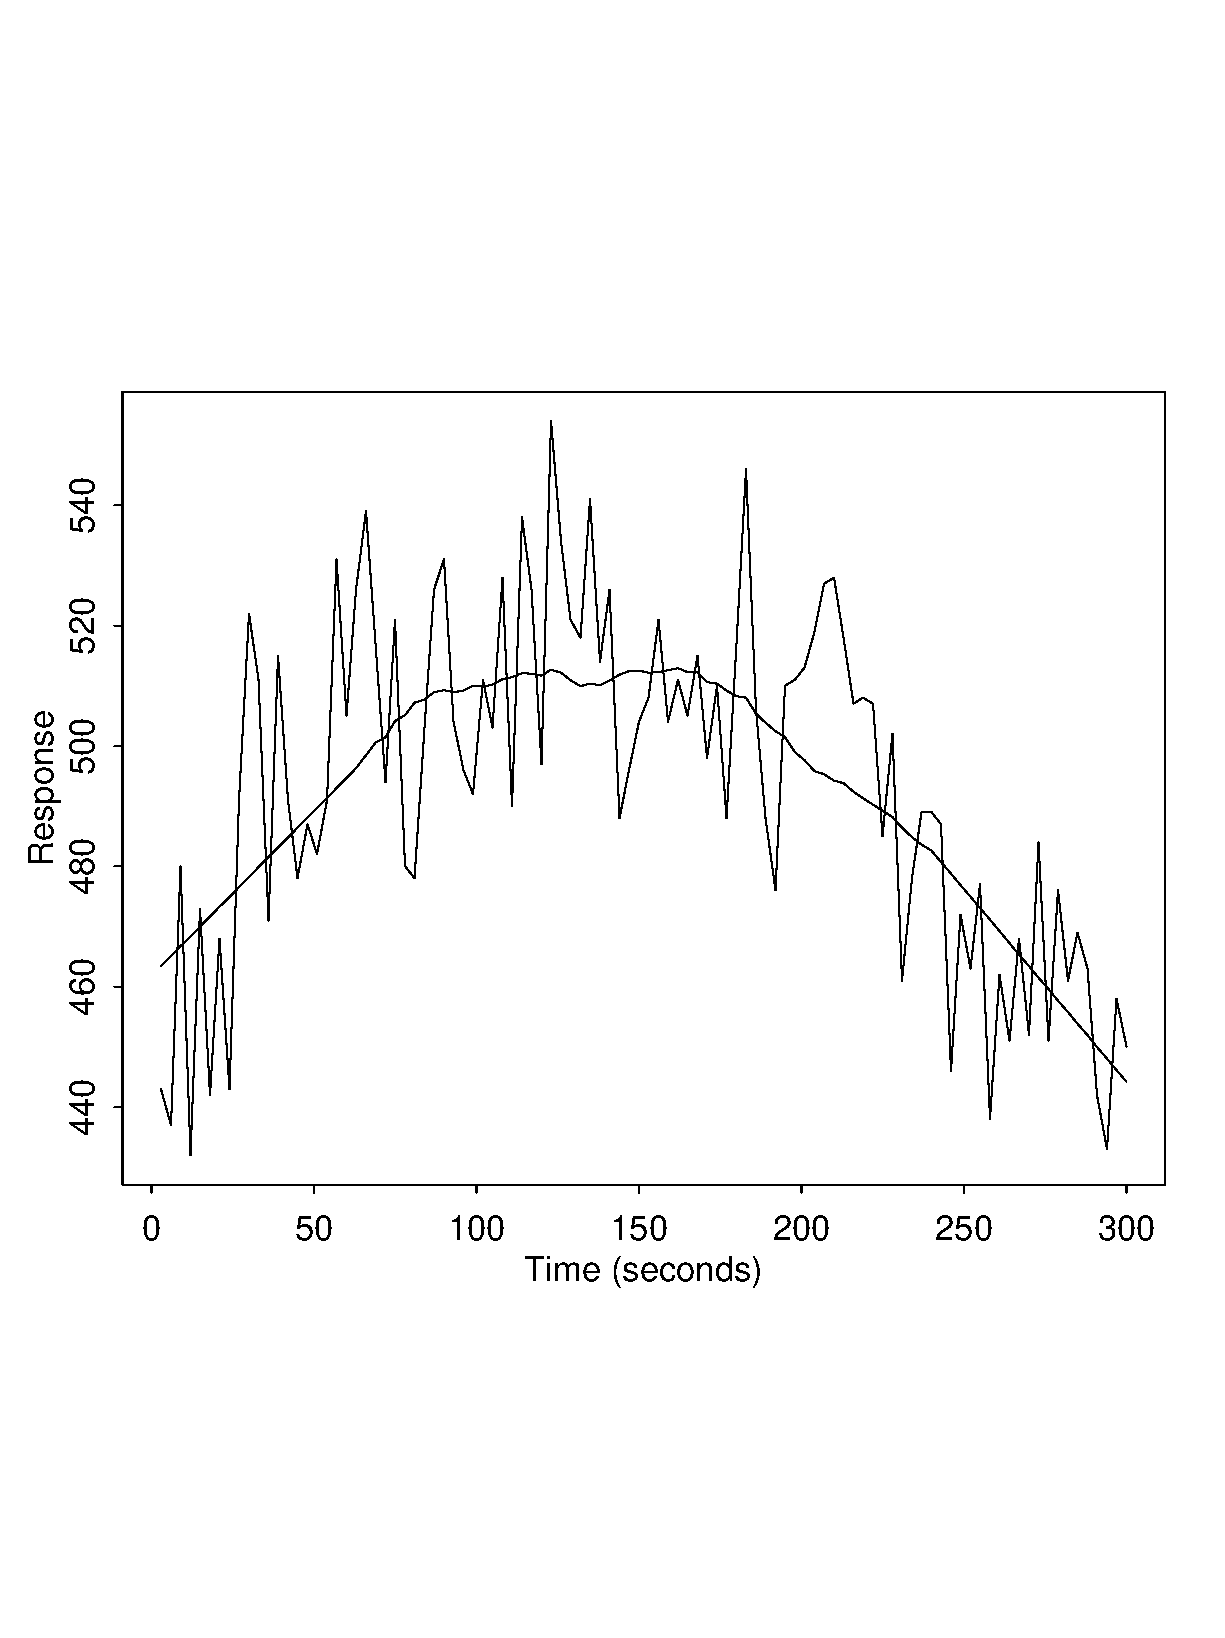
\includegraphics[height=90mm,bb=25 169 579 595]{jm.fig3.eps}
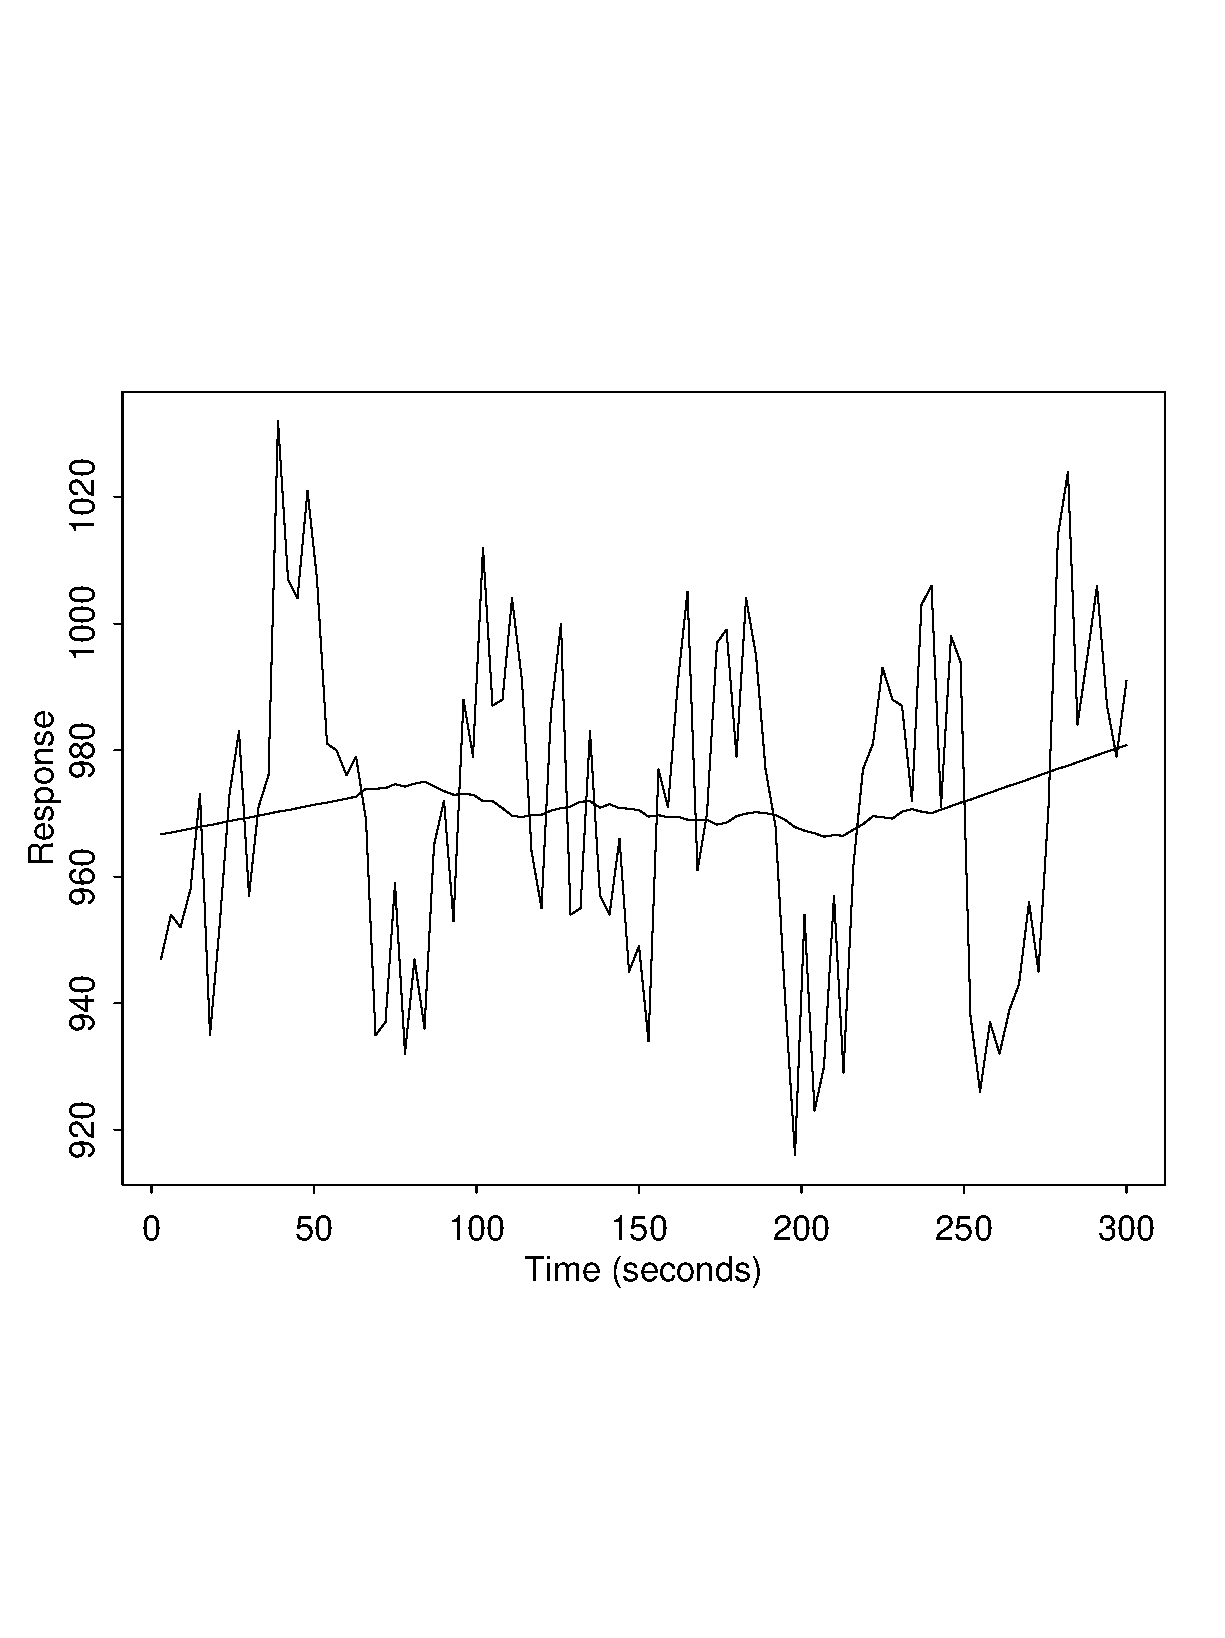
\includegraphics[height=90mm,bb=25 169 579 595]{jm.fig2.eps}
  \caption{Trend Removal:(left) }
\label{trends}
\end{figure}


%% Column 2. (Just indicative, multicols distributes text automatically)

\section{Theory}
The asymptotic sampling properties of the periodogram are well-known \cite{priestley:1981}.
For increasingly long series:
\begin{itemize}
\item $I(\omega_j)/f(\omega_j) \sim \textrm{E}$ where E has a
  standard exponential distribution.
\item $I(\omega_j)$ and $I(\omega_k)$ are independent for all
  $k\ne j$.
\end{itemize}
where $f(\omega)$ is the spectral density of the underlying stationary stochastic process.
This is a very general result, includes AR, MA and ARMA processes as special cases and is known to be accurate for series of moderate
length, such as those encountered in fMRI experiments. If we assume that the underlying spectral
density $f(\omega)$ is smooth then we can use a smoothed version of
$I(\omega)$, which we denote $g(\omega)$, to estimate $f(\omega)$.




\section{Testing for a response to the stimulus}

The spectral density estimate provides us with a baseline against
which to test for significant departures from the underlying process.
From (I),
\begin{colorequation}
  \frac{I(\omega_j)}{f(\omega_j)} \sim E
\label{eq:13}
\end{colorequation}
Substituting $g(\omega_j)$ for $f(\omega_j)$, we define the ratio
statistic, $R_j$, as
\begin{colorequation}
  R_j = \frac{I(\omega_j)}{g(\omega_j)},\qquad\qquad \omega_j=j/\delta
  n
\label{eq:14}
\end{colorequation}
By calculating the statistic $R_j$ at the fundamental frequency of
activation, $\omega_c$, we obtain a test statistic, $R_c$, for
significant activation. Large values of $R_c$ indicate a large effect at the fundamental
frequency. All of the statistics $R_j$, apart from $j=0$ and $n/2$, will have the same distribution as $R_c$ and thus can be used as a benchmark against which to compare the theoretical distribution of $R_c$, at negligible computational cost. Thus the method is effectively self-calibrating.

\begin{figure}
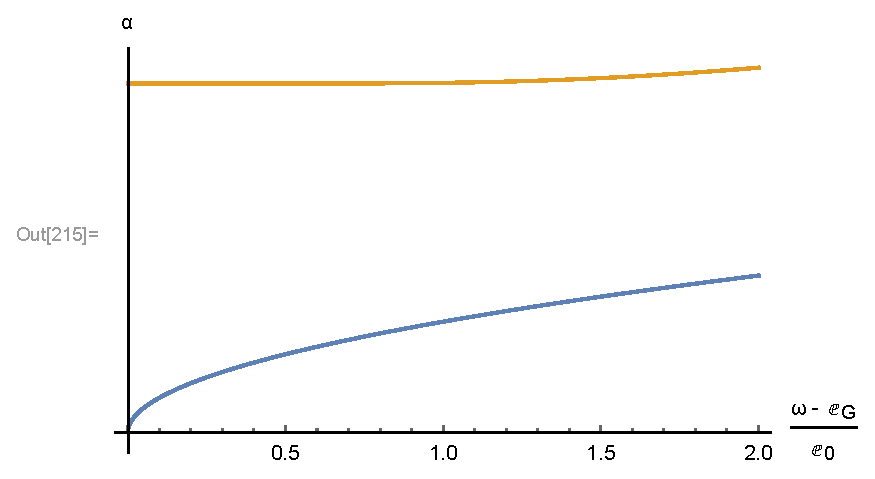
\includegraphics[height=160mm,bb=100 285 500
    570]{AbsFinal.eps}
\caption{$p$-value maps thresholded at $10^{-4}$ obtained using our approach (left) and an AR(1) approach (right)}
\label{vis}          
\end{figure}

\begin{figure}
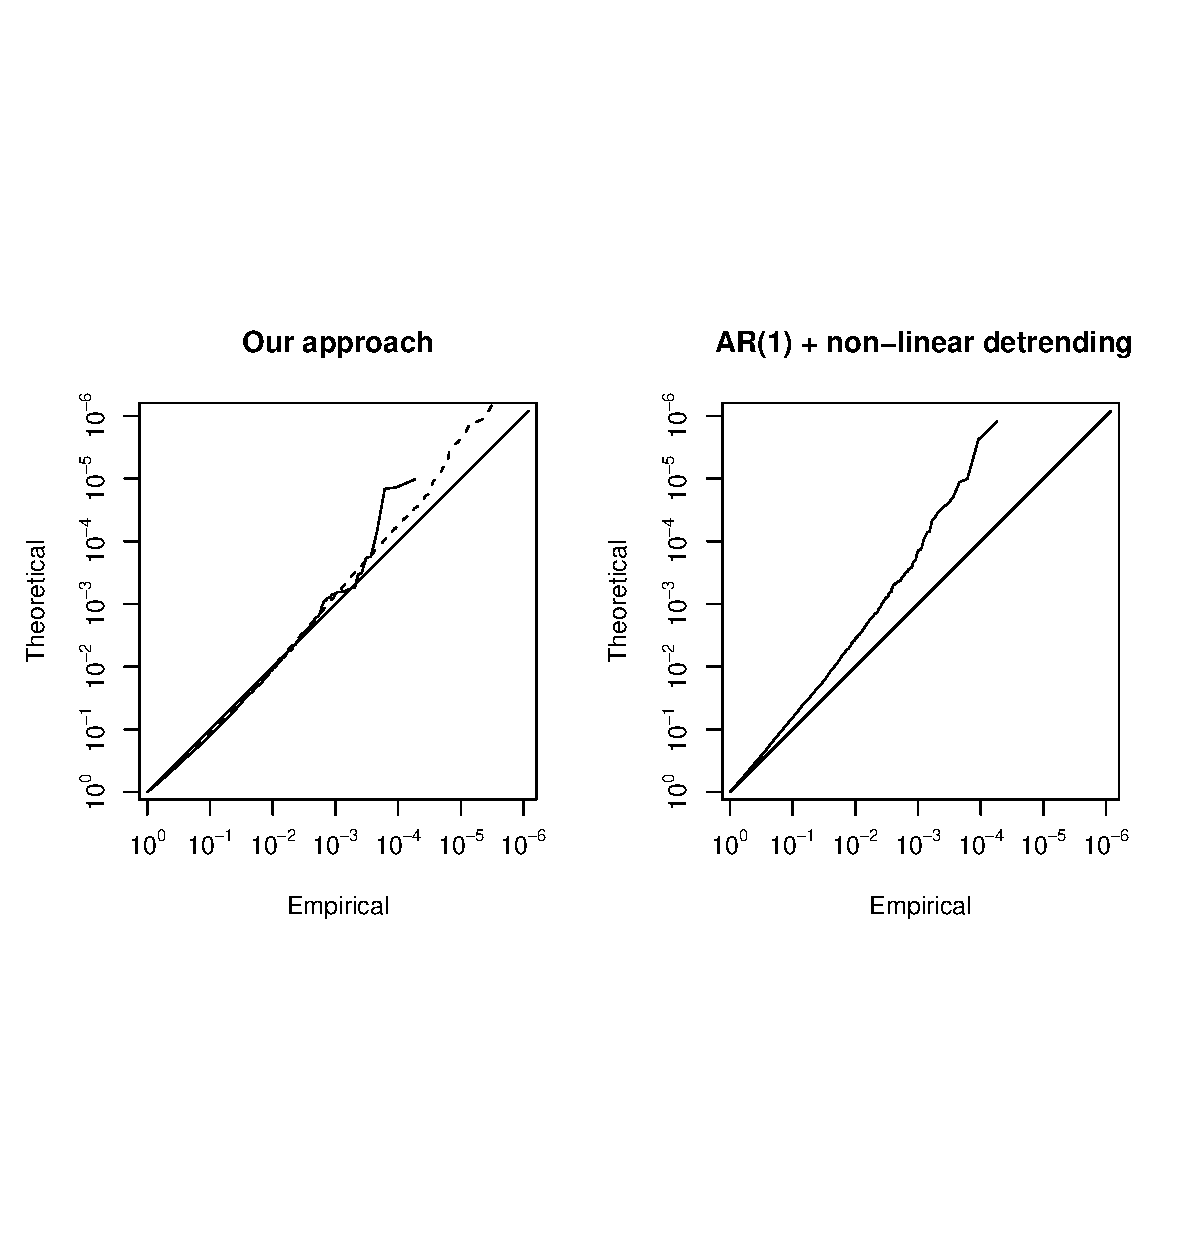
\includegraphics[height=220mm,bb=18 270 570 770]{null.pp.ps}
%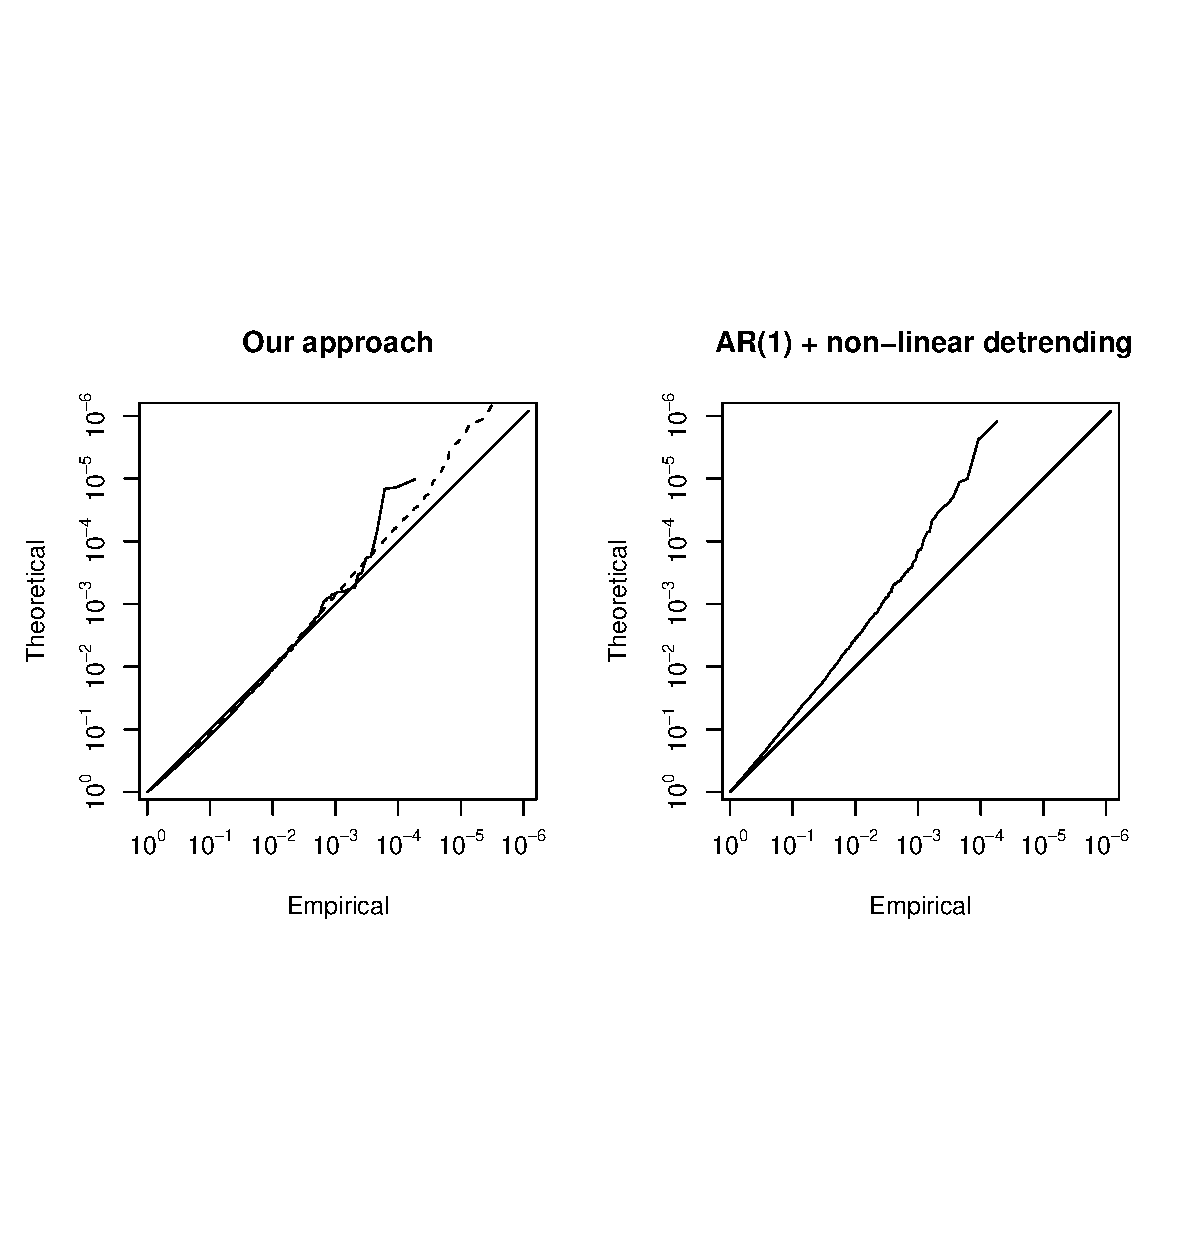
\includegraphics[height=90mm,bb=23 140 555 700]{null.pp.ps}
\caption{$PP$-plots for our approach (left) and an AR(1) approach (right) applied to a null dataset}
\label{pp.plots}          
\end{figure}

%% Column 3. (Just indicative, multicols distributes text automatically)

\section{High frequency artefacts}
In some datasets we have found high frequency artefacts that occur in narrow bands and have been attributed to Nyquist ghosting(figure~\ref{ghost} (right)). We have detected these artefacts using our values of $R_j$ at high frequencies (figure~\ref{ghost} (left) shows a thresholded $R_{88}$ image).
\begin{figure}
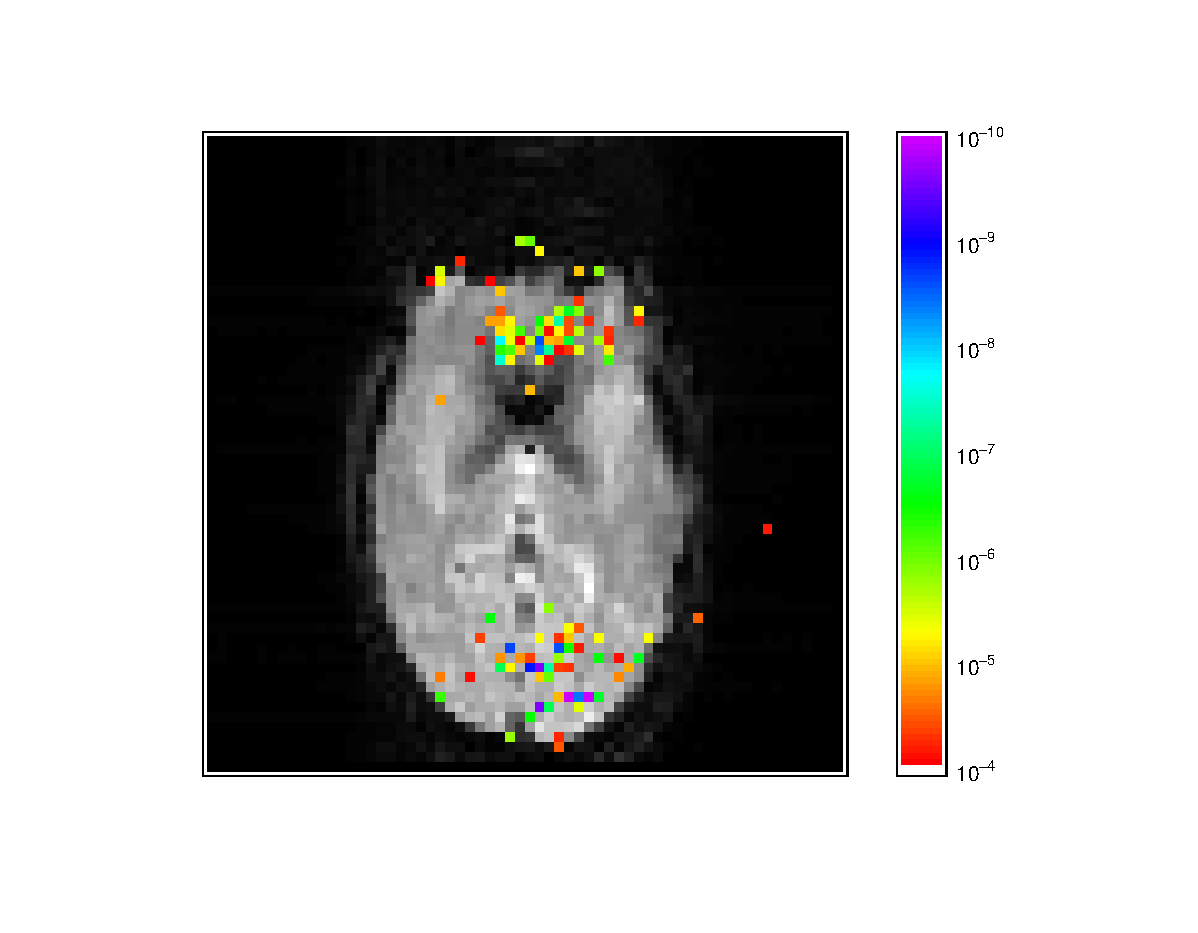
\includegraphics[height=80mm,bb=100 265 500 590]{jm.fig19.eps}
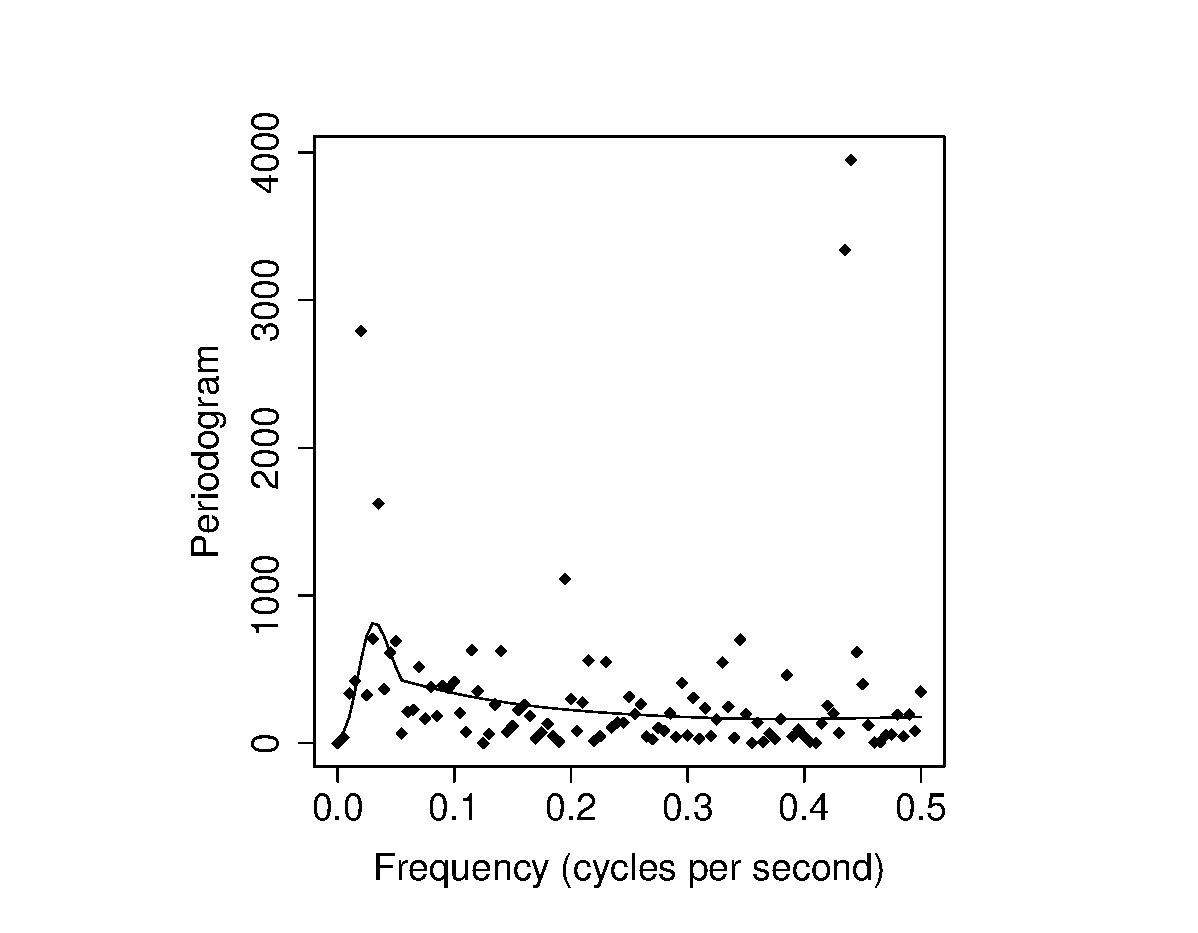
\includegraphics[height=90mm,bb=90 210 470 600]{jm.fig17.eps}
\caption{}
\label{ghost}
\end{figure}
We have found that parametric-time domain models may be extremely susceptible to these artefacts whereas non-parametric spectral density estimation will be resistant. Three methods were applied to a voxel in an area exhibiting the high-frequency artefact. Method I: The AR(1) approach described above, Method II: As Method I but with high frequency artefact removed, Method III: Our approach. Comparing Method I and II, in the table below, we see that the estimated parameters are significantly different after the artefact has been removed, which results in a misleading statistic. Even after removal, there is no guarantee that the AR(1) model is flexible enough and this results in the difference between Methods II and III.
\begin{center}
\small
\begin{tabular}{|l||c|c|c|c|c|}
\hline 
& AR(1) coefficient & $\widehat{\sigma^2}$ & Numerator & Denominator & Ratio Statistic\\
\hline \hline
Method I & $-$0.0027 & 15765 & 591.88 & 315.29 & 1.877\\
\hline
Method II & 0.2839 & 11276 & 624.98 & 419.46 & 1.490\\
\hline 
Method III& --- & --- & 689.30 & 513.88 & 1.341\\
\hline 
\end{tabular}
\end{center}


\section{Conclusion and extensions}

Non-parametric spectral estimation is shown to be an accurate and self-calibrating approach for analyzing periodic designs. The method makes few assumptions and is resistant to high-frequency artefacts whereas parametric time-domain approaches may be susceptible to these artefacts and biased by the assumptions they make on the form of the spectral density. The method can be easily extended to handle non-periodic event related designs and initial results are extremely promising.
Non-parametric spectral estimation is shown to be an accurate and self-calibrating approach for analyzing periodic designs. 


\section{Acknowledgements} 
We are grateful to Dr Stephen Smith (fMRIB Centre, Oxford) for
advice and datasets.

%---------------------------------------------------------------------------
% --- Bibliography
%---------------------------------------------------------------------------

\bibliographystyle{plain}
\bibliography{jm.ref}


\end{multicols}

% Make a footer line/box:
\makefooter

\end{document}





